\chapter{Methode}\label{ch:Methode}

% Hier halten Sie fest und begründen, welches Vorgehensmodell Sie für Ihr Projekt wählen. Sie
% verweisen allenfalls auf die daraus entstandenen, konkreten Terminpläne mit Meilensteinen, welche
% z.B. unter Realisierung (Kapitel 5) oder im Anhang versorgt sind.
% Bei Projekten mit einer verlangten wissenschaftlichen Tiefe werden hier die geplanten
% Forschungsmethoden wie quantitative/qualitative Interviews, Befragungen, Beobachtungen,
% Feldexperiment etc. beschrieben und begründet.
% Warum ist in Ihrer Situation ein Interview besser als eine Umfrage? Wer soll interview werden?
% 2(Sie können bei Bedarf in Absprache mit Ihrer Betreuungsperson dazu auch ein zusätzliches
% Methodencoaching beziehen).
% Bei Engineering-Projekten halten Sie weitere einzusetzende fachliche Methoden oder Techniken fest.
% Bei einem Softwareprojekt können dies z.B. der geplante Einsatz einer Anforderungsanalyse, der
% Einsatz von Review-Techniken (Architektur-Reviews) oder bekannter Programmiertechniken sein.
% Dazu gehört auch eine Teststrategie (wo setzen Sie im Projekt Schwerpunkte betr. Testen?). Die
% eigentliche Testdurchführung ist dann unter Realisierung, im Anhang oder einem selbstständigen
% Testdokument beschrieben.

% TODO Nach eigenen Bedürfnissen erweitern
% ------------------------------------- TEIL Wissenschaftliche Arbeiten ----------------------------------------------------
\subsection{Laborexperiment}
% quantitaiv, ehter verhaltenswissenschaftlich als konstruktiv

% Das Experiment untersucht Kausalzusammenhängein kontrollierter Umgebung, indem
% eine Experimen-talvariable auf wiederholbare Weise manipuliert unddie Wirkung
% der Manipulation gemessen wird. DerUntersuchungsgegenstand wird entweder in
% seiner na-türlichen Umgebung (im »Feld«) oder in künstlicherUmgebung (im
% »Labor«) untersucht, wodurch wesentlichdie Möglichkeiten der Umgebungskontrolle
% beeinflusstwerden. (Balzert, S. 286)

% ------------------------------------- TEIL Ingenieurlastige Arbeiten ----------------------------------------------------
\section{Projektinformationen}

In diesem Abschnitt wird aufgezeigt welches Vorgehensmodell und welche Methoden verwendet wurden zur Abwicklung dieses Projektes.
Auch wird aufgezeigt wie das Projekt organisiert ist.

\subsection{Vorgehensmodell}

 In den Besprechungen hat sich ergeben, dass wir inkrementell und iterativ arbeiten möchten
(siehe Anhang~\ref{sec:meeting_03_03_2021}, Abschnitt ''Projektmanagementmethode).
Das Projektmanagement soll schlank gehalten werden und nicht viel Aufwand erzeugen, auch da ich alleine an diesem Bericht arbeite.

Dementsprechend habe ich als Vorgehensmodell wurde Kanban ausgewählt.

Folgendes sind einige Kernpraktiken von Kanban kurz erklärt:

\begin{enumerate}
    \item \textbf{Arbeit sichtbar machen}: Arbeit muss sichtbar gemacht werden, um zu sehen wo der Arbeitsfluss im Gesamtsystem stockt.
        Auch arbeitet man bei Kanban nicht nach dem Push-Prinzip sondern dem Pull-Prinzip. Das 
        Das heisst es wird keine Arbeit zugewiesen, sondern neue Arbeit wird abgeholt sobald die letzte Aufgabe (oder Issue/Task) fertiggestellt wurde.
    \item \textbf{Limitiere den Work in Progress (WIP)}: Es ist schwierig ständig zwischen Aufgaben zu wechseln. Deshalb soll nur an einer Aufgabe auf einmal gearbeitet werden. Tritt ein Problem auf bei einer Aufgabe, legt man diese auf die Seite, um diese später mit jemandem anzuschauen, oder erledigt erst eine andere Aufgabe welche eine Voraussetzung ist.
    \item \textbf{Manage Flow}: Arbeitsfluss ist wichtig in Kanban. Es soll Aufmerksamkeit gelegt werden auf Engpässe oder gar Blockaden im System. Dabei hilft es zu unterscheiden was für verschiedene Arbeitstypen das Team erledigen muss und das verschiedene Arbeiten einen anderen Grad an Dringlichkeit haben.
    \item \textbf{Explizite Prozessregeln}: Die Regeln sollen offen gelegt und explizit gemacht werden, damit man merkt wann diese gebrochen oder nicht mehr sinnvoll sind.
    \item \textbf{Feedback Mechanismen}: Um die Arbeitsprozesse kontinuierlich verbessern zu können, benötigt es Feedback-Mechanismen. Dies kann z.B. an täglichen Stand-Ups oder an Retrospektiven. Dies sind Meetings wo darauf abgezielt wird dazuzulernen, den Arbeitsprozess zu reflektieren und  zu Verbessern.
\end{enumerate}

(\cite[p.~17-22]{siegfried_kaltenecker_kanban_2013})

\subsection{Projektorganisation}

\subsubsection{Projektteam}

Die folgende Tabelle~\ref{tab:projectmembers} listet alle Personen auf die an diesem Projekt beteiligt sind.

\begin{table}[H]
    \begin{tabular}{l p{3.2cm}}
        \toprule
        \bfseries Person   & \bfseries Rollen \\
        \midrule
        Konrad Bächler     & Auftraggeber \\
        \midrule
        Carolyn Bächler    & Auftraggeber \\
        \midrule
        Arnold Dieter      & Betreuungsperson \\
        \midrule
        tbd.               & Experte \\
        % TODO: find out who's the expert
        \midrule
        Moritz Küttel      & Student \\
        \bottomrule
    \end{tabular}
    \caption{People involved in the project}\label{tab:projectmembers}
\end{table}

\subsubsection{Quellcode}

Der \LaTeX-Quellcode für diesen Bericht ist auf codeberg.org in diesem Repository zu finden:
\url{https://codeberg.org/mkuettel/ba}

%TODO: add links to all the source code

\subsubsection{Projektboard und Issue-Tracker}

Die Abbildung~\ref{fig:projectboard} zeigt das Projektboard, welches für Projektmanagement und Controlling verwendet wird.
Jede Karte auf dem Projektboard ist eine Aufgabe oder auch Issue aus dem folgenden Issue-Tracker:

\url{https://codeberg.org/mkuettel/ba/issues}

Der Issue-Tracker ist zugleich ein Backlog. Issues können nach Bedarf aus dem Issue-Tracker entnommen werden und zum Projektboard hinzugefügt werden.

Das Projektboard ist ein Kanban-Board und enthält drei Spalten: ''To Do'', ''In Progress'' und ''Done''.
Diese Issues aus dem Issue-Tracker können dann je nach fortschritt in die Spalten einsortiert werden. 
Ziel von Kanban ist es eines nach dem anderen zu machen und sich auf einen Task zu fokussieren. Man sollte also nie mehr als einen Issue in der Spalte ''In Progress'' haben.
%TODO: definition of done
% https://de.wikipedia.org/wiki/Kanban_(Softwareentwicklung)

%TODO: describe how issues are categorized (labels, milestones, projects etc.)

Das Kanban-Board ist hier zu finden:

\url{https://codeberg.org/mkuettel/BA/projects/125}



\begin{figure*}[ht]
    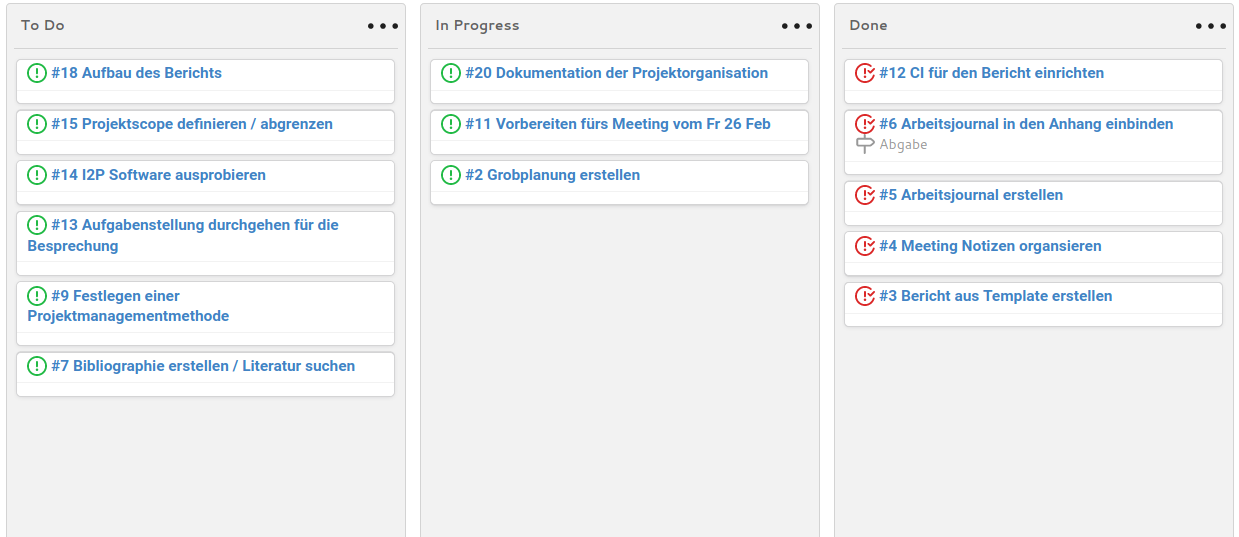
\includegraphics[width=1.0\textwidth]{project-board.png}
    \caption{CodeBerg Project Board}
    \label{fig:projectboard}
\end{figure*}


Ein einziger Issue sollte nie mehr Aufwand machen als acht Stunden Arbeit. Diese Regel hilft die Issues kleiner zu halten und genauere Aussagen treffen zu können, wo man im Projekt steht.

Wird an einem Issue gearbeitet wird dies im Journal vermerkt \& in der Git-Historie hinterlegt.
Das Arbeitsjournal ist im Anhang~\ref{sec:journal} zu finden.


Die Länge eines Sprints in Kanban ist nicht genau definiert, sondern der Sprint ist fertig wenn alle Arbeit für den jeweiligen Sprint erledigt wurde.

\subsection{Ermittlung offener Projektrahmenbedingungen}
\label{sub:RequirementsEngineering}

Zweimal pro Woche trifft sich das Projektteam wo Fragen und das Weitere
Vorgehen besprochen wird. Es wird jeweils ein Meeting-Protokoll erstellt (siehe
Anhang~\ref{ch:meetingnotes}), worin festgehalten wird was besprochen wurde.

Die Anforderungen entspringen nun aus diesen Diskussionen und Protokollen und sowie aus der Aufgabenstellung.
Auch Vorgaben der Hochschule Luzern wurden als Anforderung aufgenommen.

Fragen bezüglich Anforderungen werden jeweils als Traktanden für das nächste Meeting aufgenommen und dann Besprochen oder direkt mit dem Auftraggeber geklärt.

Für die Liste von Anforderungen siehe Abschnitt~\ref{sec:Anforderungen}.


\subsection{Projektanforderungen / Anforderungsanalyse}
\label{sub:Anforderungen}

Die Anforderungen an das Projekt haben sich aus der Aufgabenstellung (siehe Appendix~\ref{ch:assignment}) sowie aus dem Requirement Engineering (siehe Dazu den Abschnitt~\ref{sub:RequirementsEngineering}).

Die folgende Tabelle~\ref{tab:requirements} zeigt alle Anforderungen auf.
Die erste Spalte ''Id'' gibt jeder Anforderung einen eindeutigen Kennzeichner, um diese einfacher zu Referenzieren.
Die Anforderung selber ist in der Spalte ''Anforderung'' genauer beschrieben.
Die Spalte ''Art'' gibt an, ob es sich bei der Anforderung um eine funktionale oder nicht-funktionale Anforderung handelt.
Nicht jede Anforderung muss zwingend erfüllt werden. Deshalb kennzeichnet die Spalte ''Optional'', ob die jeweilige Anforderung zwingend erfüllt werden muss.

\newcommand*{\reqref}[1]{
    \hyperref[{req:#1}]{\ref{req:#1}-#1}
}
\newcommand*{\seereq}[1]{(siehe Anforderung \reqref{#1})}
\newcommand*{\rid}[1]{\label{req:#1}-#1}
\begin{longtable}{N p{8.5cm} l l}
    \toprule
    \multicolumn{1}{r}{\bfseries Id} & \bfseries Anforderung                                                                                                                                                           & \bfseries Art & \bfseries Optional \\ \midrule
    \endhead
    \rid{SDTF}  & Der Stand der Technik/Forschung muss ermittelt werden und in den Bericht eingebunden werden.
                & Nicht Funktional & Nein  \\ \midrule


    \rid{TINF}  & Es ein Teststand muss aufgebaut werden welches es erlaubt verschiedene Performance-Messungen
                  an einem Netzwerk bestehend mehreren i2pd-Knoten. & Funktional & Nein \\ \midrule
    \rid{TKON}  & Es soll ein Konzept erstellt werden für den Teststand, wie dieser aussehen soll, wie er funktioniert und was genau gemessen werden soll. & Nicht-Funktional & Ja \\ \midrule
    \rid{TREP}  & Die am Teststand durchgeführten Messungen sollten so gut wie möglich reproduzierbar sein. Die gleiche Messung sollte soweit wie möglich dieselben Resultate liefern. & Nicht-Funktional & Nein \\ \midrule
    \rid{TCNF}  & Der Teststand muss konfigurierbar sein (inwiefern?), damit verschiedene Messungen durchgeführt werden können.  & Funktional & Nein \\ \midrule
    \rid{TSCL}  & Das Testnetzwerk soll zwischen 8 Knoten bis maximal 256 i2pd-Knoten unterstützen. Dies muss konfigurierbar sein, dass Testnetzwerk sollte skalieren können. & Funktional & Nein \\ \midrule
    \rid{TISO}  & Das Testnetzwerk soll isoliert sein vom realen I2P-Netzwerk. & Nicht-Funktional & Nein \\ \midrule
    \rid{TLAT}  & Die Latenz von Nachrichten die über das I2P-Testnetzwerk gesendet werden, soll gemessen werden. & Funktional & Nein \\ \midrule
    \rid{TLIM}  & Es muss möglich sein im Teststand die verfügbare Bandbreite von einzelnen i2pd-Knoten einzustellen. & Funktional & Nein \\ \midrule
    \rid{TVRS}  & Man soll schnell (wie schnell?) ein neues Experiment mit neuen Einstellungen starten können. & Nicht-Funktional & Nein \\ \midrule
    \rid{EVAL}  & Die am Teststand durchgeführten Messungen müssen evaluiert und aufgearbeitet werden.  & Nicht Funktional & Nein \\ \midrule
    \rid{TPER}  & Man geht davon aus das die Messungen lange dauern könnten, da jeweils ein ganzes Netzwerk und dessen Traffic erstellt und gehandhabt werden muss. Es macht Sinn die Ausführungszeiten von Messungen kurz zu halten, damit mehr Messungen durchgeführt werden können. & Nicht-Funktional & Ja \\ \midrule
    \rid{DOCS}  & Am Ende des Projekts muss dieser Bachelorarbeit abgegeben werden. Dieser Bericht soll das Projekt, die verwendeten Methoden, Evaluationsprozesse, die Umsetzung und Resultate beschreiben.
                & Nicht Funktional & Nein \\ \midrule
    \rid{ITER}  & Ein iteratives Projektmanagement wird bevorzugt für kurze Feedback-Zyklen. Da ich alleine am Projekt arbeite sollte so auch weniger Overhead entstehen. & Nicht Funktional & Ja \\ \midrule
    \rid{PRES}  & Es muss eine Zwischenpräsentation gehalten werden, welche das Projekt und das weitere Vorgehen erklärt.
                & Nicht Funktional & Nein \\ \midrule
    \rid{WEBA}  & Es muss ein Web-Abstract erstellt werden, der das Projekt kurz zusammenfasst. Der Web-Abstract wird veröffentlicht und muss eine Woche vor Projektende vom Betreuer abgenommen werden.
                & Nicht Funktional & Nein \\ \midrule
    \rid{PVID}  & Es muss ein 90 Sekunden Video erstellt werden, welches diese Bachelorarbeit kurz erklärt. Das Video wird am Start der Schlusspräsentation abgespielt.
                & Nicht Funktional & Nein \\ \midrule
    \bottomrule
    \caption{Requirements}\label{tab:requirements}
\end{longtable}

\subsection{Einschränkungen und Abgrenzungen}

Es soll nur die Performance des I2P-Netzwerks mit der i2pd-Software untersucht werden und nicht von darüberliegenden Applikationen.

% TODO: Scope in der Einleitung
% TODO: Scope definieren

\subsection{Planung}
\label{sec:Planung}

Für diese Bachelorarbeit werden 360 Stunden Arbeit während den 15. Projektwochen geleistet.
Im Schnitt bedeutet dies acht Stunden Arbeit an jeweils 3 Wochentagen (meistens jeweils Mittwoch-Freitag).

% 15 Wochen * 3 Tage * 8h = 360h

\subsubsection{Meilensteine}
\label{sec:meilensteine}

Die Meilensteine sind im Projektkalender (\fullref{tab:projektkalender}) hellblau gekennzeichnet und hier aufgelistet.

\begin{enumerate}
    \item \textbf{Startdatum}: Mittwoch 24. Februar 2021, Kick-Off-Meeting
    \item \textbf{Zwischenpräsentation}: 14. April 2021
    \item \textbf{Abgabe Web-Abstract}: 21. Mai 2021
    \item \textbf{Abgabedatum}: 4. Juni 2021
    \item \textbf{Schlusspräsentation}: 13.6 - 3.7 2021
\end{enumerate}

Die Meilensteine sollen ein Controlling-Mechanismus, um zu merken, wann das Projekt im Verzug ist.
An den jeweiligen Meilensteine müssen folgende Resultate erzeugt worden sein:


Diese Meilensteine wurden auch in den Issue-Tracker aufgenommen:

\url{https://codeberg.org/mkuettel/BA/milestones}

\subsubsection{Phasen}
\label{sec:phasen}

Das Projekt wird in 4 Phasen durchgeführt die im der \fullref{tab:projektkalender} aufgezeigt sind.
Dabei sind die Phasen jeweils durch Meilensteine voneinander abgegrenzt.

\begin{enumerate}
    \item \textbf{Konzeptionsphase}: Die Konzeptionsphase beginnt mit dem Kick-Off Meeting
        In dieser Phase wird das Projekt geplant, recherchiert, der Bericht wird strukturiert, die Anforderungen werden eruiert und  ein Konzept für einen Teststand wird erstellt.
    \item \textbf{Aufbau des Teststands}: Ein Teststand aufbauen nach Konzept um Performance-Experimente und Messungen mit der i2pd-Software in einem Netzwerk machen zu können.
Analyze what needs to be tested and determine testing criteria, create a test plan.
    \item \textbf{Auswertungsphase}: Verschiedene Performance-Experimente und Messungen werden in dieser Phase ausgeführt und ausgewertet.
    \item \textbf{Abschlussphase}: Vervollständigen des Berichts, Fazit erstellen, Korrekturlesen, Erstellung des Web-Abstracts.
\end{enumerate}


\subsubsection{Projektkalender}

Regelmässige Meetings finden jeweils am Mittwoch Morgen, am Start der Projektwoche, und am Freitag Morgen.

Die Spalte ''PW'' gibt die Projektwoche an. Die Spalte ''KW'' die Kalenderwoche.

\newcommand{\cellblue}[1]{\cellcolor{cyan} #1}
\begin{table}[H]
    \begin{tabular}{r r l l|c c|c c c|c c}
        \toprule
         \textbf{PW} & \textbf{K}      & \textbf{Phase} & \textbf{Meilensteine} & \multicolumn{7}{c}{\textbf{Wochentag}} \\
               &            &                       &                       & Mo                                      & Di & Mi  & Do & Fr & Sa & So \\ \midrule
                           &                         &                       &                       & \multicolumn{7}{c}{\textit{Februar}}   \\
          1                & 8                       & \textbf{Konzeption}         & Projektstart          & 22                                      & 23 & \cellblue{24}  & 25 & 26 & 27 & 28 \\
          2                & 9                       &                       &                       & 29                                      & 30 & 31 \\
          |                & |                       &                       &                       &                                        \\
          |                & |                       &                       &                       & \multicolumn{7}{c}{\textit{März}}      \\
          3                & 9                       &                       &                       & 1                                       & 2  & 3   & 4  & 5  & 6  & 7  \\
          4                & 10                      &                       &                       & 8                                       & 9  & 10  & 11 & 12 & 13 & 14 \\
          5                & 1                       &                       & 1. Konzept Teststand     & 15                                      & 16 & 17  & 18 & 19 & 20 & 21 \\
          \midrule
          6                & 12                      & \textbf{Aufbau des}          &                       & 22                                      & 23 & 24  & 25 & 26 & 27 & 28 \\
          7                & 13                      & \textbf{Teststands}            &                       & 29                                      & 30 & 31  &    &    &    &    \\
          |                & |                       &                       &                       &                                        \\
          |                & |                       &                       &                       & \multicolumn{7}{c}{\textit{April}}     \\
          7                & 14                      &                       &                       &                                         &    &     & 1  & 2  & 3  & 4  \\
          8                & 15                      &                       &                       & 5                                       & 6  & 7   & 8  & 9  & 10 & 11 \\
          9                & 16                      &                       & 2. Zwischenpräsentation  & 12                                      & 13 & \cellblue{14}  & 15 & 16 & 17 & 18 \\
          \midrule
          10               & 17                      & \textbf{Auswertung}         &                       & 19                                      & 20 & 21  & 22 & 23 & 24 & 25 \\
          11               & 18                      &                       &                       & 26                                      & 27 & 28  & 29 & 30 &    &    \\
          |                & |                       &                       &                       &                                        \\
          |                & |                       &                       &                       & \multicolumn{7}{c}{\textit{Mai}}       \\
          11               & 18                      &                       &                       &                                         &    &     &    &    & 1  & 2  \\
          12               & 19                      &                       & 3. Auswertung            & 3                                       & 4  & 5   & 6  & 7  & 8  & 9  \\
          \midrule
          13               & 20                      & \textbf{Abschluss}             &                       & 10                                      & 11 & 12  & 13 & 14 & 15 & 16 \\
          14               & 21                      &                       & 4. Web-Abstract          & 17                                      & 18 & 19  & 20 & \cellblue{21} & 22 & 23 \\
          15               & 22                      &                       &                       & 31                                      &    &     &    &    &    &    \\
                           & |                       &                       &                       &                                        \\
                           & |                       &                       &                       & \multicolumn{7}{c}{\textit{Juni}}      \\
          15               & 23                      &                       & 5. Abgabe                &                                         & 1  & 2   & 3  & \cellblue{4} & 5  & 6  \\
        \bottomrule
    \end{tabular}

    \caption{Projektkalender}
    \label{tab:projektkalender}
\end{table}

Es gilt zu beachten das dies eine Planung ist, wie das Projekt effektiv verlaufen ist ist ersichtlich aus dem Issue-Tracker und dem Arbeitsjournal im Anhang~\ref{sec:journal}.


